\section{MVP Functionality}

The instruction needs to be compliant with section 14.6.1 of the OpenGL 4.6 Core Specification. The polygon rasterization stage just describes the inner loop of rasterization. However, the process described can just be repeated for each triangle in the scene. 
The instruction aims to implement both loops of the rasterization algorithm. This reduces flexibility of the block but can provide massive performance gain by accelerating the outer loop in hardware. I imagine that a great deal of the design work done to accelerate the out loop will be to design high throughput data transfer of triangles from memory to the unit.

The system can be described using \Cref{algorithm:FinalPseudoCode}, where the steps referred to in the code refer to parts of \Cref{sec:rasterOpenGL}.

\begin{algorithm}
\caption{An algorithm with caption}\label{algorithm:FinalPseudoCode}
\begin{algorithmic}
    \For{Triangle Strip in Scene}
        \State Split Strip into individual triangles
        \For{Set of individual triangles}
            \If{Triangle is back-facing}
                \State Cull triangle
            \Else
                \State Generate Bounding Box
                \For{Pixel in bounding box}
                    \State Create Fragment
                    \If{anti-aliasing}
                        \State Calculate fragment attributes using interpolation with anti-aliasing
                    
                    \Else
                        \State Calculate fragment attributes using interpolation 
                    \EndIf
                \EndFor
                    \State Write fragment to fragment array
            \EndIf
        \EndFor
    \EndFor
\end{algorithmic}
\end{algorithm}

\section{Instruction Format}
The minimum viable product for this project would be to add a single instruction to the RISC-V 32G ISA that implements the pseudocode in \Cref{algorithm:FinalPseudoCode} using hardware.

I plan to use the following instruction format for my design:

\begin{verbatim}
    rasterizeTriangleStrip riI, riV, roF, resX, resY, CR0, CR1

\end{verbatim}

Where the parameters are:


\begin{itemize}
    \item[\textbf{riI}]: Pointer to Index array of ints stored in a register
    \item[\textbf{riV}]: Pointer to Vertex array stored in a register
    \item[\textbf{roF}]: Pointer to Fragment array stored in a register
    \item[\textbf{resX}]: the horizontal resolution of the monitor
    \item[\textbf{resY}]: the vertical resolution of the monitor
    \item[\textbf{CR0}]: a control register that contains the values of the relevant flags, described in \Cref{sec:rasterOpenGL}
    \item[\textbf{CR1}]: the same as CR0, contains additional flags that do not fit in CR0
\end{itemize}
These registers will need to be set before the instruction is called. This would be done using \textit{mov} or any other instruction that places its results in a register.


\subsection{Inputs}
\subsubsection{Vertex Array}
Let the number of supported generic vertex attributes (the value of MAX\_VERTEX\_ATTRIBS) be n. (section 10.6 of OpenGL spec)
Array of 4 element generic vertex attributes, the first element always being the vertex coordinates, the array will therefore take the format shown by \Cref{fig:VertexArrayFormat}.

\begin{figure}[ht]
    \centering
    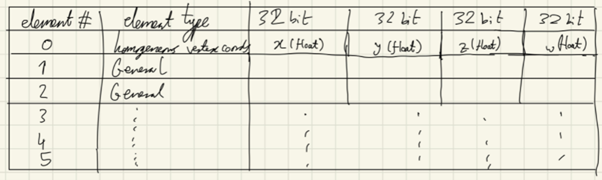
\includegraphics{functional_spec/images/VertexArrayFormat.png}
    \caption{Caption}
    \label{fig:VertexArrayFormat}
\end{figure}
\subsubsection{Index Array}
The index array will just be an array of integers which correspond to the indicies of the vertices being referred to in the vertex array. Important to note is that the index array will be interpreted as storing a set of triangle strips.

\subsubsection{Registers}
We will also need to decide where the input/output registers will be located.
\paragraph{\textbf{Design Decision: Where will the instruction input registers be located?}}

The options are shown in \Cref{tab:GPRvsNewReg}.
\begin{table}[ht]
\begin{tabular}{|l|l|l|}
\hline
\textbf{Options}                                                                          & \textbf{Pros}                                                                                                                                                                                       & \textbf{Cons}                                                                                                       \\ \hline
\begin{tabular}[c]{@{}l@{}}Put them in general \\ purpose registers \\ (GPR)\end{tabular} & \begin{tabular}[c]{@{}l@{}}- Simplifies the design\\ - Less work needs to be done to the decode \\   unit and compiler to support the new \\   registers\end{tabular}                               & \begin{tabular}[c]{@{}l@{}}- There are fewer registers \\   available \\   to the rest of the program.\end{tabular} \\ \hline
Create new registers                                                                      & \begin{tabular}[c]{@{}l@{}}- More registers are available to the rest \\   of the program\\ - Process for adding these registers can be \\   documented and used for future extensions\end{tabular} & \begin{tabular}[c]{@{}l@{}}- Complicates the design of \\   the system significantly\end{tabular}                   \\ \hline
\end{tabular}
\caption{}
\label{tab:GPRvsNewReg}
\end{table}

\begin{shaded}\label{decision:GPRvsNewReg}

Creating a new set of registers significantly complicates the modification of the existing core as shown in \Cref{tab:GPRvsNewReg}. Even if they mean the design is set up to be more extensible for future work, it is not worth risking the completion of the project.
\newline
\newline
\textbf{Conclusion: GPR's will be used for inputs to the rasterizer.}
\end{shaded}

\subsubsection{Image Resolution}
\textbf{Design Decision: How will image resolution be set?} \newline
One thing to note is that the simplest way to provide the monitor resolution to the hardware unit is by  or otherwise. This however is rather clunky and makes programs written for the rasterizer less flexible since they will need to be changed and recompiled if image resolution needs to change. 

Another more complex option is to query the monitor for its resolution by asking for its Extended Display Identification Data (EDID)\cite{EDIDExplanation}. This is a data structure is a standardised means for a display to communicate its capabilities to a source device. This may be considered as an extension once the MVP has been delivered.

\begin{table}[ht]
\begin{tabular}{|l|l|l|}
\hline
\textbf{Options}                                                                                       & \textbf{Pros}                                                                                                                                                                         & \textbf{Cons}                                                                                                                                     \\ \hline
\begin{tabular}[c]{@{}l@{}}Direct input by\\ setting input \\ registers in the \\ program\end{tabular} & \begin{tabular}[c]{@{}l@{}}- Simplifies the design since\\ hardware doesn't need to be designed \\ to query the monitor\end{tabular}                                                  & \begin{tabular}[c]{@{}l@{}}- Programs written for the \\ rasterizer are less flexible\end{tabular}                                                \\ \hline
\begin{tabular}[c]{@{}l@{}}Ask the display\\ for its EDID\end{tabular}                                 & \begin{tabular}[c]{@{}l@{}}- Programs written for the system are \\ more portable since they do not need\\ to be recompiled every time the display\\  resolution changes\end{tabular} & \begin{tabular}[c]{@{}l@{}}- Complicates the design of \\  the system since new hardware \\ must be designed to query the \\ monitor\end{tabular} \\ \hline
\end{tabular}
\caption{}
\label{tab:monitorResInput}
\end{table}
\begin{shaded}\label{decision:monitorResInput}
For an academic project like this one, the portability of the software is not particularly import and so image resolution will be provided through direct input to the instruction. However, this is a very important feature for video display systems to have and so would make for a high priority small, extension to the project.
\newline
\newline
\textbf{Conclusion: Resolution will be provided through direct input to the instruction.}
\end{shaded}

\subsection{Outputs}
Each fragment in the fragment array will take the same format as vertices in the vertex array, although it is likely that the fragment array will be much larger than the vertex array. This must be considered when choosing the size of the system memory and will be discussed in section 
%\todo{What do other GPU’s produce as output here to make them OpenGL compliant?}
\begin{itemize}
    \item[\textbf{roF}]: Pointer to Fragment array, the fragment array can be accesses by the RISC-V CPU core for further fragment processing.
\end{itemize}

The rasterizer subsystem will write to the area allocated as the fragment array and that is the only output it will have. 

\subsection{Read-Write (RW) and Write-Read (WR) Hazards}
The instruction being implemented has many inputs and outputs and affects large areas of memory. Therefore prevention of RW and WR hazards is critical.

To prevent these hazards, memory operations that access memory used by the rasterizer should be completed before the rasterizer starts it operation. This can be done using a fence instruction from the RISC-V \textit{Zifencei} extension\cite{RVISAManualVol1}. There are available in the RISC-V "G" extension, presenting another reason for the use of RV32G.

This means that when using the \textit{rasterizeTriangleStrip} instruction, a fence must always be placed before it. 

These hazards of instructions that write to the input registers of \textit{rasterizeTriangleStrip} also need to be prevented. This is already done for normal instructions in an out of order CPU using register renaming and reservation stations. I therefore will need to modify these systems to also work with the new instruction.
